\documentclass[12pt]{article}


%\setcounter{section}{-1}
% Style guide
% Each 'section' is a chapter (PDF) on Brightspace
% Each 'subsection' is one of those slides with the headings all faded except the one we're now starting
% Each slide is a bold heading with bullet points
% Numerous headings on a similar topic may be grouped into sub-sub-sections discretionarily
% They are 1-indexed in accordance with the notes on BS

\usepackage{enumitem}
\usepackage{amsmath}
\usepackage{parskip}
\usepackage{outlines}
\usepackage{framed}
\usepackage{graphicx}
\usepackage{xcolor}
\pagecolor{black}
\color{white}

\begin{document}

\tableofcontents

\begin{flushright}[Lecture on 1.2]\end{flushright}

\section{Introduction}
Dr. Declan Delaney

\subsection{Motivation and Introduction}
\begin{outline}[enumerate]
\1 Signals travel without wires
    \2 In this module, signals travel as radio waves\\
    (optical and acoustic systems ignored)
\1 Applications are mostly in communications
    \2 Signals modulated to carry information
    \2 Many familiar applications such as radar, navigation, etc.
\end{outline}

\begin{framed}
Example: Modern smart phone has approximately 9 distinct wireless systems. Try identifying them?


\begin{itemize}[noitemsep]
    \item NFC
    \item Cellulars
    \begin{itemize}[noitemsep]
        \item 2G
        \item 3G
        \item 4G
        \item 5G
    \end{itemize}
    \item GPS
    \item Bluetooth
    \item WiFi
    \item UWB
    \item Lidar
\end{itemize}
\end{framed}

\textbf{Advantages of Wireless}

\begin{itemize}[noitemsep]
    \item Mobility
    \item Good for one-to-many transmissions
    \item Cheap
\end{itemize}
Increasingly used for high capacity point-to-point links (cheaper than wired) (e.g. to serve remote areas)

\textbf{Advantages of Wired}

\begin{itemize}[noitemsep]
    \item Very little leakage
    \item No interference
    \item Multiple systems can operate adjacently without issue
\end{itemize}
but considerably more overheads.
Suitable for super high capacity lines (eg. fibre-optic transatlantic cables)

\subsection{The Wireless Spectrum}
The EM spectrum is a shared and limited resource.\\
Mostly regulated by government agencies.

Frequencies must be carefully given out, but can be reused at different locations as we will see.

Overview of a wireless system:
\begin{itemize}[noitemsep]
\item Start with raw data
\item Source coding (compression)
\item Channel coding (error detection \& error correction)
\item Modulation
\item TX
\item RX
\item Demodulation
\item Channel decoding
\item Source decoding
\end{itemize}

This module is mainly about modulation and TX/RX, the rest is information theory.

\subsection{Assessment \& Delivery}
    \begin{tabular}{ l l l }
        \textbf{Component} & \textbf{Timing} & \textbf{Weight} \\
        Lab Assignments & Varied (3 labs) & 25\% \\
        Online BS quizzes & ? & 25\% \\
        Final Exam & & 50\%
    \end{tabular}


\begin{itemize}[noitemsep]
    \item Lab 1: Receiver architectures
    \item Lab 2: Phase-Locked Loops
    \item Lab 3: Amplifiers
\end{itemize}


Open book final with emphasis on design and problem solving

\subsection{Module Outline}

\begin{itemize}[noitemsep]
    \item (1) Radio Link Design
    \begin{itemize}[noitemsep]
        \item Link budget?
        \item How far? How much power?
    \end{itemize}
    \item (2) Non-Linear System
    \item (3) Frequency Generation and Synthesis
    \item (4) Transmitter Design
    \begin{itemize}[noitemsep]
        \item Requirements and specifications
        \item Transmitter architecture choices
    \end{itemize}
    \item (5) Noise
    \begin{itemize}[noitemsep]
        \item Sources of noise
        \item Noise analysis, low-noise design
    \end{itemize}
    \item (6) Receiver Design
    \begin{itemize}[noitemsep]
        \item Requirements and specifications
        \item Receiver architecture choices
    \end{itemize}
    \item (7) Transceiver Design
    \begin{itemize}[noitemsep]
        \item Transmitter and receiver combined!
    \end{itemize}
    \item (8) Antennas and Propagation
    \begin{itemize}[noitemsep]
        \item Review of antenna theory
        \item Practical antennas and propagation of radio waves
    \end{itemize}
    \item (9) System-Level Issues and Examples
\end{itemize}

\subsection{Textbooks}
Purely optional, module notes should be sufficient.

\begin{itemize}[noitemsep]
    \item "Microwave and RF Design of Wireless Systems"

    by David M. Pozar
    \item "Antennas"

    by John D. Kraus
\end{itemize}

\begin{flushright}[Lecture on 1.3]\end{flushright}

\subsection{Basics of Wireless Communication}
Amplifier to increase signal power enough to drive the antenna

\textbf{Multiple Access}
\begin{itemize}[noitemsep]
\item CSMA: Listen to the channel, send if it's clear
\item FDMA: Frequency divided MA
\item TDMA: Time divided MA
\end{itemize}

You require a 'guard band' between frequency bands where no data is sent to avoid interference

CDMA is a good way to overcome this waste, ODMA is an even better approach

\subsubsection{Main components of a transmitter}
\begin{itemize}[noitemsep]
    \item Signal is 'mixed' (modulated) with an oscillator at the frequency of the channel being used
    \begin{itemize}[noitemsep]
        \item The frequency has to be adjustable to allow for different channels
    \end{itemize}
    \item A power amp is required to power an antenna
\end{itemize}
Amp goes first because high-frequency amplification is a fucking nightmare

\subsubsection{Main components of a receiver}
Signal arrives on an antenna (which collects EM waves in the vicinity, sometimes in a preferred direction, and puts them on a cable, waveguide, or circuit board track)

RX:
\begin{itemize}[noitemsep]
    \item Receive at very low power
    \item Select and amplify the desired signal
    \item Estimate the original signal
\end{itemize}

The signal is too weak to demodulate, so you need a high-frequency amplifier before the demodulator.

For most of this module, we will look at block-level circuits and not worry about precise circuit design.

Channel capacity (Shannon-Hartley):
\begin{math}
C = B \times\text{log}_2(1+\frac{S}{N})
\end{math}

\begin{itemize}[noitemsep]
    \item C is channel capacity (eg. bits per second)
    \item B is bandwidth (Hz)
    \item $\frac{S}{N}$ is the signal-to-noise ratio
\end{itemize}

Cellular:
\begin{itemize}[noitemsep]
    \item 2G operated at 800-900 MHz and 64 kHz channels
    \item 3G operated at 1-2 GHz and got 8 MHz channels
    \item 4G operates at up to 5 GHz and 50-100 MHz channels
    \item 5G has channels up to 10 GHz
\end{itemize}
The increase in speed is partially due to better MA schemes, but mainly due to the bigger bandwidth.

Other options to increase capacity:
\begin{itemize}[noitemsep]
    \item Increase SNR
    \begin{itemize}[noitemsep]
        \item Increase power (limited by regulations)
        \item or reduce noise (choose a frequency with less background?)
    \end{itemize}
\end{itemize}

\section{Basic Antennae \& Propagation}
\subsection{Basic Antennae}
\textbf{Radio link design}
\begin{itemize}[noitemsep]
    \item What will be the power at the receiver (or SNR)?
    \item How far away can the antennae be?
    \item How much power is needed?
\end{itemize}
Answers culminate in a \textit{link budget} calculation

\textbf{Antennae}
\begin{itemize}[noitemsep]
    \item Circuitry generates the signal and amplifies to high power
    \item High power signal goes along a 'feed track'
    \begin{itemize}[noitemsep]
        \item Very little losses here
    \end{itemize}
    \item Then into the antenna
    \begin{itemize}[noitemsep]
        \item Can be directed, but not guided, so loses power quickly
        \item Not all power is radiated, some is lost
    \end{itemize}
\end{itemize}

\begin{flushright}[Lecture on 1.5]\end{flushright}

\textbf{Antenna Power}

Ignoring free space losses
\begin{itemize}[noitemsep]
    \item Assume total power remains constant as it propagates
    \item but spreads over a larger area (inverse square law)
    \item Consider \textit{power density} in $W/m^2$
\end{itemize}

With space losses
\begin{itemize}[noitemsep]
    \item Model with a 'propagation constant' $\gamma \ge 2$
    \item \begin{math}
    \frac{\text{Power density at distance }r_2}{\text{Power density at distance }r_1} = \frac{r_1}{r_2}^\gamma
    \end{math}
\end{itemize}

\textbf{Isotropic Reference Antenna}
\begin{itemize}[noitemsep]
    \item Assume a point source
    \item Radiates in all directions uniformly
    \item 100\% of input power is radiated
\end{itemize}
Not possible but useful for comparison purposes

\textbf{Omni-directional Antenna}
\begin{itemize}[noitemsep]
    \item Similar model but losses are allowable
    \item I npractice only possible in one plane
\end{itemize}

\textbf{Antenna Gain}
\begin{itemize}[noitemsep]
    \item Antennae are not amps - they don't actually have gain.
    \item However, a focused antenna delivers more power to the receiver than an isotropic tradiator, so there is a 'focusing gain'\\[1em]

    \begin{math}
    \text{Gain in a particular direction} := \frac{\text{Power density observed in that direction}}{\text{Power density expected from an isotropic radiator}}
    \end{math}\\[1em]

    \item Obviously normally measured in the direction of transmission
\end{itemize}

\subsubsection{Receiver Antennae}

\begin{itemize}[noitemsep]
    \item Collects electromagnetic waves
    \item May be directional - sensitive to waves from a certain direction
    \item Measure the aperture / collection area
    \begin{itemize}[noitemsep]
        \item Some antennae have an obvious physical aperture (eg. parabolic dish)
        \item Others have an 'effective aperture' $A$, such that
        \begin{math}
        P_{RX} = D_{RX}A
        \end{math}
        where $P_{RX}$ is the collected power and $D_{RX}$ is the power density of the incoming wave
        \end{itemize}
    \item Aperture efficiency
    \begin{itemize}[noitemsep]
        \item Even those with a physical aperture have an 'effective aperture', which is lower due to losses on the dish\\
        \begin{math}
            \text{Aperture efficiency} := \frac{\text{Effective aperture } A}{\text{Physical aperture}} < 1
        \end{math}
    \end{itemize}
    \item Always use 'effective aperture', which accounts for dish losses
\end{itemize}

\textbf{Reciprocity}

\begin{itemize}[noitemsep]
    \item Antennae can TX and RX
    \begin{itemize}[noitemsep]
        \item Same beam and shape each way
    \end{itemize}
    \item RX gain is equal to TX gain
    \item One expression for gain based on the aperture is\\
    \begin{math}
        G = \frac{4\pi A}{\lambda^2}
    \end{math}
    where $\lambda$ is wavelength.
\end{itemize}

\begin{flushright}[Lecture on 2.2]\end{flushright}

\subsection{Basic Propagation}

\begin{itemize}[noitemsep]
    \item Speed of light in free space
\end{itemize}

\textbf{Propagation on Earth}
\begin{itemize}[noitemsep]
    \item Curvature of Earth comes into play
    \item Distance to horizon is given by $d=\sqrt{h(2R+h)}\sim \sqrt{2Rh}$
    
    where $R$ is Earth's radius and $h$ is the tower height
    \item For tower-to-tower, you have to consider the height of both towers, the maximum distance between them is the sum of their distances to horizon
\end{itemize}

\textbf{Atmospheric Effects at High Frequency}
\begin{itemize}[noitemsep]
    \item Air is less dense higher up so refraction causes high frequency waves to 'bend' downward, which shortens transmission range
    \item Compensate by pointing TX upward, increasing total range!
    \item 'Effective' Earth radius $R$ becomes $\frac{4}{3} R$
\end{itemize}

\textbf{Atmospheric Effects at Low Frequency}
\begin{itemize}[noitemsep]
    \item Between 3 and 30 MHz, strong refraction in ionosphere
    \item Waves can bend back and return to Earth
    \item But propagation changes with day/night and season
\end{itemize}
\begin{figure}[h!]
    \centering
    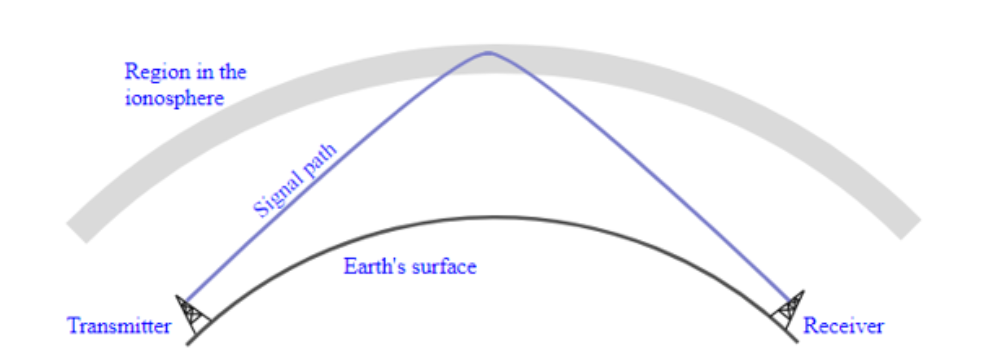
\includegraphics[width=0.5\linewidth]{images/image4.png}
    %\caption{} % Optional caption
    %\label{fig:} % Optional label for referencing
\end{figure}

Cool fact: at 3 Mz, a vertically polarised wave will curve around Earth's surface perfectly (called ground wave propagation, example is the Rugby Atomic Clock system)

\subsubsection{Free Space Links}
Consider a line-of-sight scenario
\begin{itemize}[noitemsep]
    \item Typically > 1 GHz
    \item Directional antennae on both ends
    \item No obstructions
\end{itemize}
\begin{figure}[h!]
    \centering
    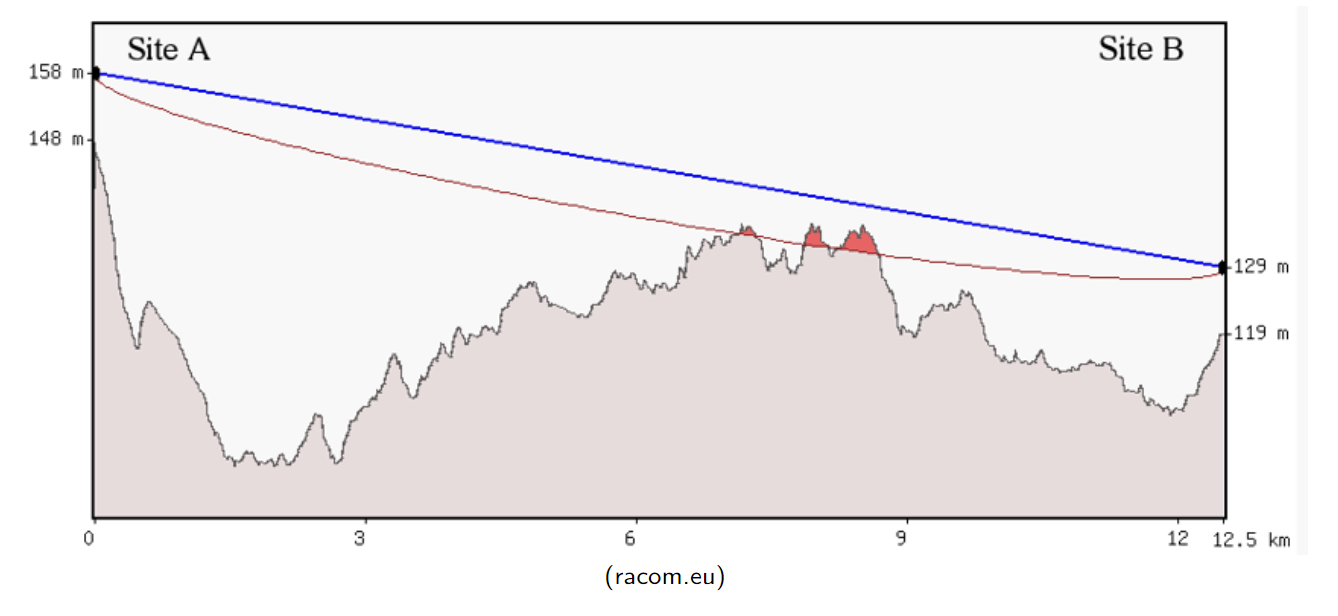
\includegraphics[width=0.5\linewidth]{images/image5.png}
    %\caption{} % Optional caption
    %\label{fig:} % Optional label for referencing
\end{figure}
This is not a suitable line-of-sight (LOS) path (blue), because the hills are \textit{close} to the LOS, which will cause reflections

Consider two paths: direct path and reflected path. Calculate the length of each and therefore the phase difference on arrival - if they are 180 degrees out of phase, the signal will be completely destroyed! Reflection causes 180 degree phase switch
Okay but isn't signal strength relevant here ?
See slide 25 in this chapter

\subsubsection{Fresnel Zones}
The $n$th Fresnel zone is the ellipsoid space around transmitters where the length of any reflected path is between $(n-1)\frac{\lambda}{2}$ and $n\frac{\lambda}{2}$ longer than the LOS path.

Accordingly, an object inside the 1st Fresnel Zone would induce a phase difference between $\pi$ and $2\pi$.

The presence of obstructions in the Fresnel zone will result in \textit{some} parts of the receiving area geting destructive interference

\begin{figure}[h!]
    \centering
    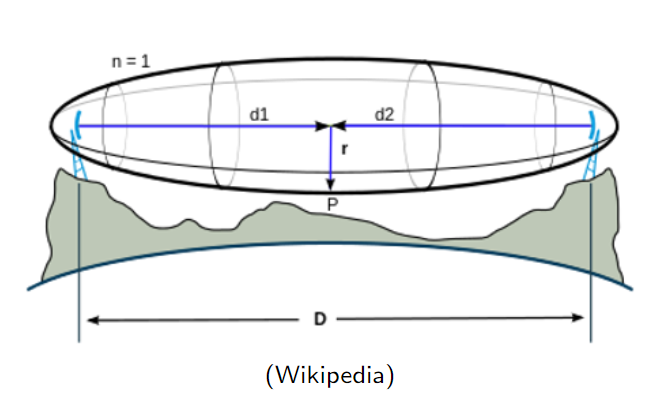
\includegraphics[width=0.5\linewidth]{images/image6.png}
    %\caption{} % Optional caption
    %\label{fig:} % Optional label for referencing
\end{figure}

Radius of the $nth$ Fresnel zone at distance $d_1$ and $d_2$ is $r_n \sim \sqrt{\frac{n\lambda d_1 d_2}{d}}$

\textbf{e.g.} For a 10 km link at 10 GHz, radius is $\sim$9 m at the centre

An object right at the edge of the Fresnel Zone actually causes constructive interference. It gets more destructive the further it goes in

Okay this makes a lot of sense but I'm losing track of the Fresnel 'layers' - is the boundary of the 2nd zone constructive or destructive ? Need to get a pen and paper and just figuer that out

Assume the reflecting surface is parallel to the LOS (anything else isn't relevant ig?)

An object in the very centre of the Fresnel Zone (parallel to the LOS) will cause perfect destructive interference (because the reflection itself causes a phase flip, and the path length will be the same)

We normally allow objects to be up to 20\% into the Fresnel zone

\subsubsection{Non-Free Space Links}

\begin{itemize}[noitemsep]
    \item In an indoor or urban landscape, there are way too many reflecting paths to use rely on Fresnel zones
    \item Variation may be rapid (e.g. high-speed trains in the way)
    \item LOS may not exist
    \item Different paths with different lengths
\end{itemize}

\section{Link Budgets}
\textbf{Contents}

\begin{itemize}[noitemsep]
    \item Computing RX signal power
    \begin{itemize}[noitemsep]
        \item Example link budget analysis
        \item Using link budget to answer design questions
    \end{itemize}
    \item Working in decibel units
    \begin{itemize}[noitemsep]
        \item Power ratio
        \item Cascade of linear systems
        \item Other dB quantities
        \item Link budget example with dB
    \end{itemize}
    \item Example broadcast satellite system
    \item Exam question Autumn 2021/22
\end{itemize}

\subsection{Computing the RX Signal Power}

\textbf{EIRP:} Effective Isotropic Radiated Power
A measure of local signal strength that answer this question: If the transmitter were an isotropic radiator (in the same place the actual antenna is), how powerful would it need to be for us to be receiving at this strength?
Measured as a power (Watts or dBW or similar)



\end{document}